\documentclass[conference]{IEEEtran}

% --- 解決 Windows 中文字型排版問題 ---
\usepackage{xeCJK}
\setCJKmainfont{MingLiU}             % 內文：新細明體
\setCJKsansfont{Microsoft JhengHei}  % 標題：微軟正黑體
\setCJKmonofont{MingLiU}
\XeTeXlinebreaklocale "zh"
\XeTeXlinebreakskip = 0pt plus 1pt
% ---------------------------------------------

\usepackage{graphicx}
\usepackage{booktabs} 
\usepackage{amsmath}
\usepackage{cite}

\begin{document}

\title{     Insertion Sort . Bubble Sort .Quick Sort: Assignment 2}

\author{\IEEEauthorblockN{馬元中}
\IEEEauthorblockA{資訊工程學系 \\
國立澎湖科技大學 \\
}}

\maketitle

\begin{abstract}
本報告旨在實作並比較三種經典排序演算法：Insertion Sort、Bubble Sort 以及 Quick Sort。透過觀察演算法在不同輸入資料規模（$n$）下之執行時間，我們驗證了其對應的時間複雜度。實驗結果證實了 $O(n \log n)$ 演算法在大數據量下的絕對優勢，同時也展示了同為 $O(n^2)$ 複雜度的演算法在常數因子與交換次數上的細微效能差異。
\end{abstract}

\section{Introduction}
排序演算法是資料結構與演算法課程中的基礎與核心。本作業延續效能分析的精神，透過親自實作（不依賴 Java 內建之 \texttt{Arrays.sort} 等工具包），探討平方時間複雜度 $O(n^2)$ 的 Insertion Sort 與 Bubble Sort，以及平均時間複雜度為線性對數 $O(n \log n)$ 的 Quick Sort。本實驗將透過真實執行數據，具象化這些演算法的擴展性（Scalability）。

\section{Algorithm Implementation}
\subsection{Methodology}
本實驗實作了三種排序演算法：
\begin{itemize}
    \item \textbf{Insertion Sort}：透過逐一將元素插入已排序區間，預期時間複雜度為 $O(n^2)$。
    \item \textbf{Bubble Sort}：透過相鄰元素兩兩比較與交換，將最大值「浮」至陣列末端，預期時間複雜度同為 $O(n^2)$。
    \item \textbf{Quick Sort}：採用分治法（Divide and Conquer），透過選定 Pivot 將陣列分割，預期平均時間複雜度為 $O(n \log n)$。
\end{itemize}
所有測試皆針對相同且隨機產生的陣列進行手動複製，以確保實驗起點的公平性，並使用 \texttt{System.nanoTime()} 計算執行毫秒數。

\section{Experimental Results}
本實驗針對規模 $n=10,000$ 至 $100,000$ 進行測試，實測數據如下表所示：

\begin{table}[htbp]
\caption{排序演算法實測執行時間 (ms)}
\centering
\begin{tabular}{crrr}
\toprule
規模 ($n$) & Insertion Sort (ms) & Bubble Sort (ms) & Quick Sort (ms) \\
\midrule
10,000  & 35.8778 & 28.7781 & 7.9181 \\
50,000  & 444.9638 & 548.2396 & 12.3987 \\
100,000 & 1737.8013 & 2141.1544 & 11.0296 \\
\bottomrule
\end{tabular}
\end{table}

\begin{figure}[htbp]
    \centering
    % 使用您指定的圖片檔名 ab
    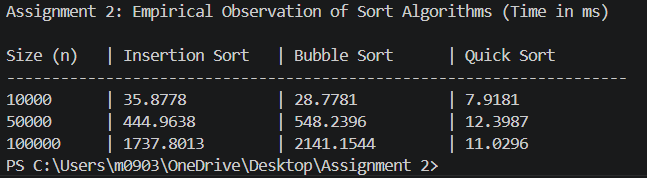
\includegraphics[width=0.48\textwidth]{ab}
    \caption{Assignment 2 執行結果實測截圖。}
    \label{fig:results}
\end{figure}

\section{Analysis and Discussion}
根據圖 \ref{fig:results} 與實測數據表，我們可得出以下深入觀察：
\begin{itemize}
    \item \textbf{$O(n^2)$ 理論驗證}：當資料量從 $10,000$ 增加 10 倍至 $100,000$ 時，Insertion Sort 的時間從 35.87 ms 成長至 1737.80 ms（約 48 倍），Bubble Sort 則從 28.77 ms 成長至 2141.15 ms（約 74 倍）。兩者皆展現了明顯的拋物線（二次方）暴增趨勢。
    \item \textbf{Insertion Sort vs. Bubble Sort}：雖然兩者理論上皆為 $O(n^2)$，但在數據量達到 100,000 時，Insertion Sort (1737 ms) 明顯快於 Bubble Sort (2141 ms)。這是因為 Bubble Sort 在最差或平均情況下需要進行極大量的元素交換（Swap），而 Insertion Sort 僅需進行元素的平移，記憶體存取成本較低。
    \item \textbf{Quick Sort 的壓倒性優勢}：在 $n=100,000$ 時，Quick Sort 僅需 11.02 ms，甚至比 $n=50,000$ 時微幅下降，這可能歸功於 JVM JIT 優化以及 $O(n \log n)$ 本身極為平緩的成長曲線。與 Bubble Sort 相比，其速度快了近 194 倍，完美印證了高效排序演算法處理大數據的必要性。
\end{itemize}

\section{Conclusion}
本實驗成功比較了三種排序演算法的效能。實測數據清楚揭示，即便在同為 $O(n^2)$ 的演算法中，常數操作（如交換次數）仍會影響實際運行時間；而 Quick Sort 的表現則再次強調了演算法複雜度等級對軟體效能的決定性影響。

\begin{thebibliography}{00}
\bibitem{b1} T. H. Cormen, C. E. Leiserson, R. L. Rivest, and C. Stein, \textit{Introduction to Algorithms}, 3rd ed. MIT Press, 2009.
\end{thebibliography}

\end{document}